% Figure: DeltaSort vs Native Sort crossover
\begin{figure}[t]
\centering
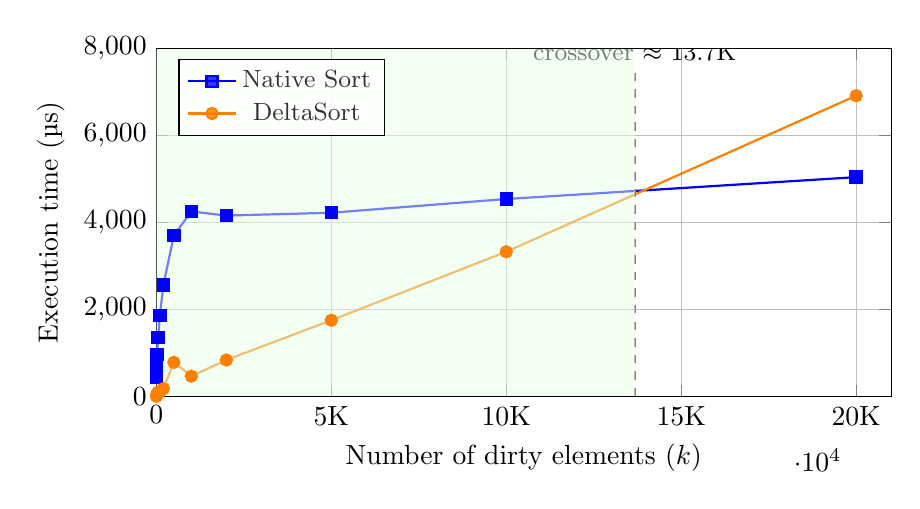
\begin{tikzpicture}
\begin{axis}[
    width=0.9\textwidth,
    height=6cm,
    xlabel={Number of dirty elements ($k$)},
    ylabel={Execution time (\textmu s)},
    xmin=0, xmax=21000,
    ymin=0, ymax=8000,
    xtick={0, 5000, 10000, 15000, 20000},
    xticklabels={0, 5K, 10K, 15K, 20K},
    ytick={0, 2000, 4000, 6000, 8000},
    legend pos=north west,
    legend style={font=\small, fill=white, fill opacity=0.8},
    grid=both,
    grid style={line width=0.1pt, draw=gray!30},
    major grid style={line width=0.2pt, draw=gray!50},
]

% Native sort (relatively flat ~4000-5000 µs)
\addplot[color=blue, mark=square*, thick, mark size=2pt] coordinates {
    (1, 439) (5, 749) (10, 747) (20, 962) (50, 1350) (100, 1867) 
    (200, 2560) (500, 3703) (1000, 4253) (2000, 4158) 
    (5000, 4223) (10000, 4539) (20000, 5042)
};

% DeltaSort (grows linearly with k)
\addplot[color=orange, mark=*, thick, mark size=2pt] coordinates {
    (1, 1) (5, 27) (10, 44) (20, 49) (50, 98) (100, 109) 
    (200, 178) (500, 782) (1000, 465) (2000, 837) 
    (5000, 1751) (10000, 3326) (20000, 6914)
};

% Crossover region annotation
\draw[dashed, thick, gray] (axis cs:13672,0) -- (axis cs:13672,7500);
\node[anchor=south, font=\small] at (axis cs:13672,7500) {crossover $\approx$ 13.7K};

% Shade the "DeltaSort wins" region
\fill[green!10, opacity=0.5] (axis cs:0,0) rectangle (axis cs:13672,8000);

\legend{Native Sort, DeltaSort}
\end{axis}
\end{tikzpicture}
\caption{DeltaSort vs.\ Native Sort for $n = 50,000$. The crossover point occurs at 
$k \approx 13,700$ (27\% of $n$). The shaded region indicates where DeltaSort is faster.}
\label{fig:crossover}
\end{figure}
